\newpage
\section{Auswertung}

\subsection{Anregung mit 405\,nm}
    \subsubsection*{Untersuchung des Kristalldurchmessers und der Polarisation}
        Die gemessenen Emissionsspektren der verschiedenen Proben werden zunächst auf die Integrationszeit und die Sensitivität des Spektrometers normiert, um vergleichbare Daten zu erhalten. Die so erhaltenen 
        Spektren sind für die drei CdSe-Nanokristallproben in Abbildung \ref{fig:size_kol} dargestellt und zeigen jeweils ein deutliches Maximum bei der Photolumineszenzwellenlänge. Um diese Wellenlänge sowie 
        die zugehörige Emissionsintensität zu bestimmen, wird an die einzelnen Spektren eine Gauß-Funktion

        \begin{equation*}
            \text{f(x)} = \text{A} \exp\left(- \frac{\left(\text{x-x}\right)_0^2}{2\sigma^2}\right)
        \end{equation*}

        angepasst.

        \FloatBarrier

        \begin{figure}[h]
        \centering
        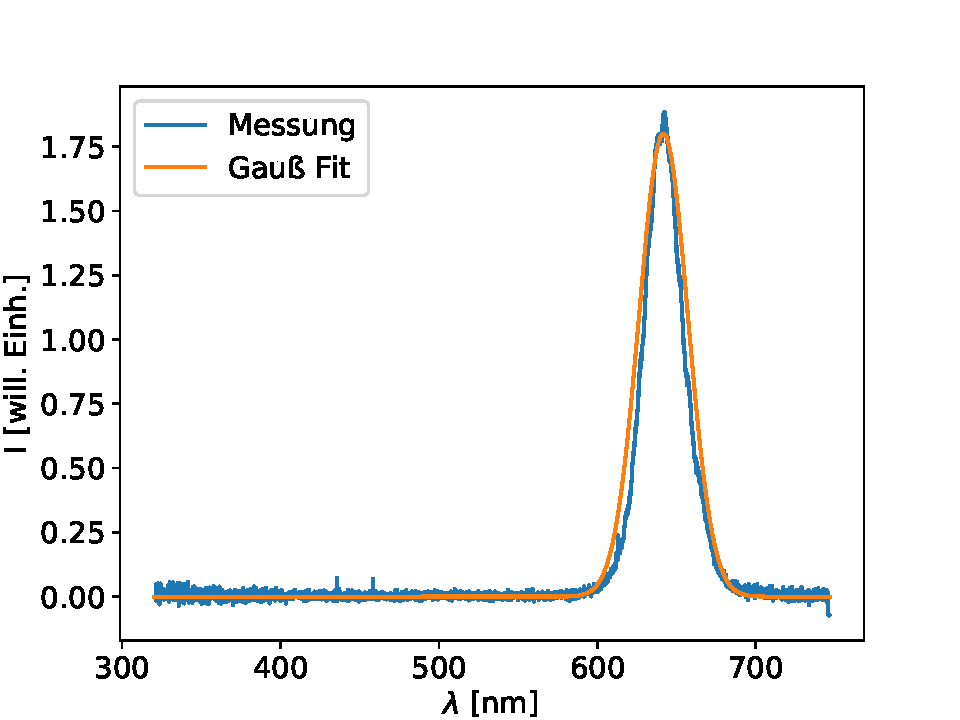
\includegraphics[width = 0.45\textwidth]{Kristall_1.pdf}
        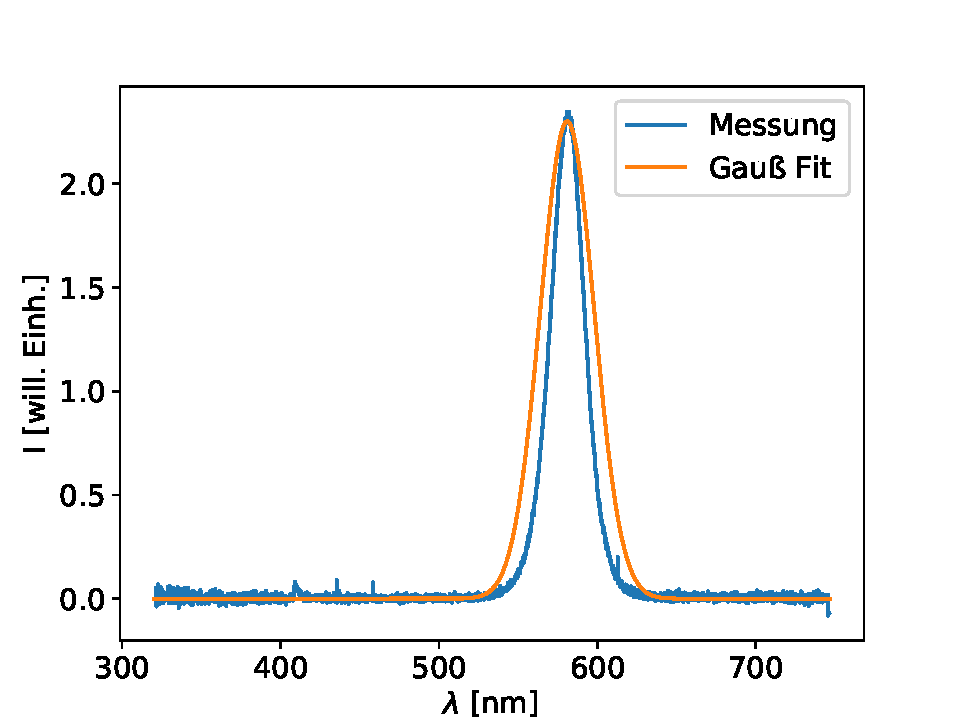
\includegraphics[width = 0.45\textwidth]{Kristall_2.pdf}
        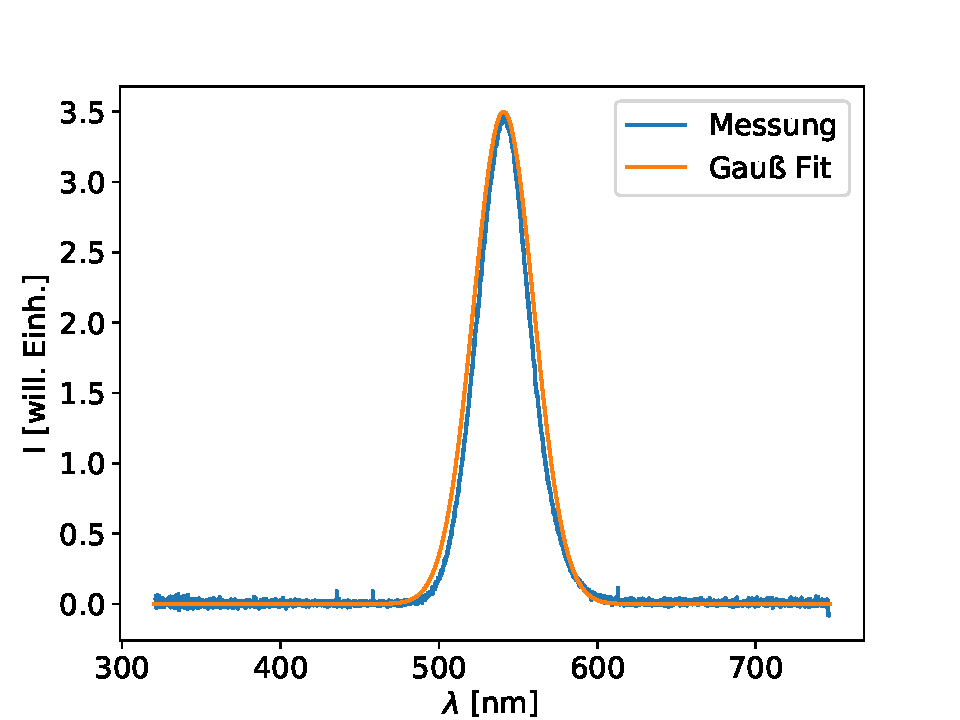
\includegraphics[width = 0.45\textwidth]{Kristall_3.pdf}
        \label{fig:size_kol}
        \caption{Verlauf der Emissionsspektren mitsamt der angepassten Gauß-Funktionen für die CdSe-Nanokristalle unterschiedlicher Größen.}
        \end{figure}

        \FloatBarrier
        \newpage
        Aus dem Parameter x$_0$, der die zentrale Emissionswellenlänge angibt, können über Formel \ref{eqn:a} und den Materialeigenschaften von CdSe 
        (\cite{tu_dortmund_versuchsanleitung_nodate-1}, \cite{foll_semiconductors_nodate}),

        \begin{center}
            \captionof{table}{Materialeigenschaften von CdSe}
            \label{tab:prop_CdSe}
            \begin{tabular}{c c}
                \toprule
                $\text{m}_{\text{e}}^*$ &  0,13$\text{m}_{\text{e}}$\\
                $\text{m}_{\text{h}}^*$ &  -0,45$\text{m}_{\text{h}}$\\
                $\text{E}_{\text{G}}$ &  \SI{1.74}{\electronvolt}\\
                $\epsilon_{\text{r}}$ &  \num{9.5}\\
                \bottomrule
            \end{tabular}
        \end{center}


        wie der effektiven Elektronenmasse $\text{m}_{\text{e}}$, der effektiven Lochmasse $\text{m}_{\text{h}}$, der Energielücke $\text{E}_{\text{G}}$ und der relativen Permittivität $\epsilon_{\text{r}}$,
        die Durchmesser a der Nanokristalle berechnet werden. Diese sind zusammen mit den Anpassungsergebnissen in Tabelle \ref{tab:Werte} aufgelistet. Da die Emissionsspektren für um 90° verschiedene 
        Polarisationen gemessen worden sind, können aus den maximalen Intensitäten der Anpassungen an die beiden Spektren unterschiedlicher Polarisation auch die Polarisationen der emittierten Strahlung 
        bestimmt werden.


        \begin{center}
            \captionof{table}{Ergebnisse}
            \label{tab:Werte}
            \begin{tabular}{c c c c c c}
                \toprule
                Probe & $\text{x}_0 $ [nm] & $\text{I}_{\text{max, 0°}}$ [a.u.] & $\text{I}_{\text{max, 90°}}$ [a.u.] & P & a [nm] \\
                \midrule
                1  & (641,74$\pm$0,14) & (1,800$\pm$0,014) & (1,800$\pm$0,014) & (0,0$\pm$0,5)\% & (2,4773$\pm$0,0018) \\
                2  & (580,99$\pm$0,14) & (2,300$\pm$0,014) & (2,300$\pm$0,014) & (0,0$\pm$0,5)\% & (1,8964$\pm$0,0010) \\
                3  & (540,85$\pm$0,14) & (3,500$\pm$0,014) & (3,500$\pm$0,014) & (0,0$\pm$0,4)\% & (1,6624$\pm$0,0010) \\

                \bottomrule
            \end{tabular}
        \end{center}

        Aus den so erhaltenen Ergebnissen wird zu einem die klare Abhängigkeit der Photolumineszenzwellenlänge von dem Nanokristalldurchmesser deutlich und zum anderen auch die nicht vorhandene Polarisation 
        des emittierten Lichts. 

    \newpage
    \subsubsection*{Abhängigkeit der Photolumineszenz von der Anregungsleistung}
        Neben der Abhängigkeit der Photolumineszenzwellenlänge von den Ausmaßen des Nanokristalls soll auch die Abhängigkeit der Photolumineszenzintensität von der Leistung des anregenden Lasers untersucht werden. 
        Dazu wird an Spektren mit Anregungsleistungen von \SI{1}{\milli\watt} bis \SI{20}{\milli\watt} jeweils die obige Gauß-Funktion angepasst und die maximale Intensität bestimmt. Diese sind in Abbildung 
        \ref{fig:IvsP} gegen die Anregungsleistung aufgetragen und zeigen deutlich einen linearen Zusammenhang, der einen Sprung bei einer Laserleistung von circa \SI{7}{\milli\watt} aufweist. 


        \FloatBarrier

        \begin{figure}[h]
        \centering
        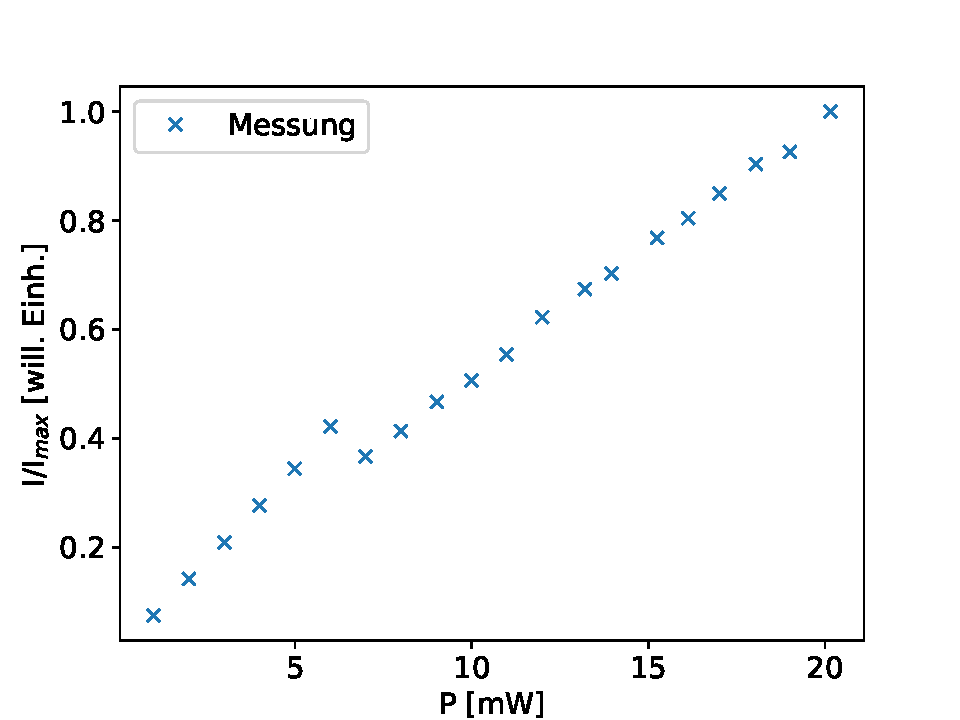
\includegraphics[width = 0.6\textwidth]{I_P.pdf}
        \caption{Angepasste maximale Intensität der Photolumineszenz gegen die anregende Laserleistung aufgetragen.}
        \label{fig:IvsP}
        \end{figure}

        \FloatBarrier


\subsection{Untersuchung mit verschiedenen Anregungswellenlängen}
    Zur Untersuchung der Photolumineszenz bei Anregung mit verschiedenen Wellenlängen wurden zusätzlich zu den Spektren bei $\lambda_{\text{Laser}}=$\SI{405}{\nano\metre} auch Spektren für Anregungsleistung
    von \SI{448}{\nano\metre}, \SI{518}{\nano\metre} und \SI{636}{\nano\metre} aufgenommen und analog auf die Spektrometereffizienz und Integrationszeit normiert. Die Spektren der verschiedenen Wellenlängen 
    sind für die vier verschiedenen Proben in Abbildung \ref{fig:PLvsLambda} dargestellt. In all diesen Spektren sind teils dünne Maxima zu erkennen. Bei diesen handelt es sich um Reflexionen des anregenden
    Lasers in das Spektrometers, da die Wellenlänge dieser Maxima exakt auf der Anregungswellenlängen liegen.
    Für den CdSe Nanokristall der Größe \SI{2.48}{\nano\metre} (o.l.) ist für alle Anregungswellenlängen Photolumineszenz zu beobachten. Die Intensität der lumineszenten Strahlung sinkt dabei mit sinkender 
    Anregungsenergie sprich steigender Wellenlänge. Für die Kristalle der Größen \SI{1.90}{\nano\metre} (o.r.) und \SI{1.66}{\nano\metre} (u.l.) ist der Laser mit der niedrigsten Energie nicht mehr dazu in der Lage 
    Elektronen in das Leitungsband anzuregen und es tritt keine Photolumineszenz auf. Dies hängt mit der aus Formel \ref{eqn:a} ersichtlichen größeren Energie eines Exzitons bei kleinerem 
    Nanokristalldurchmesser zusammen. Die Kohlenstoffprobe konnte nur von den zwei Lasern der höheren Energie zu Photolumineszenz angeregt werden. Die dabei entstehenden Peaks sind im Vergleich zu den der 
    CdSe-Nanokristalle deultich breiter.


    \FloatBarrier

    \begin{figure}[h]
    \centering
    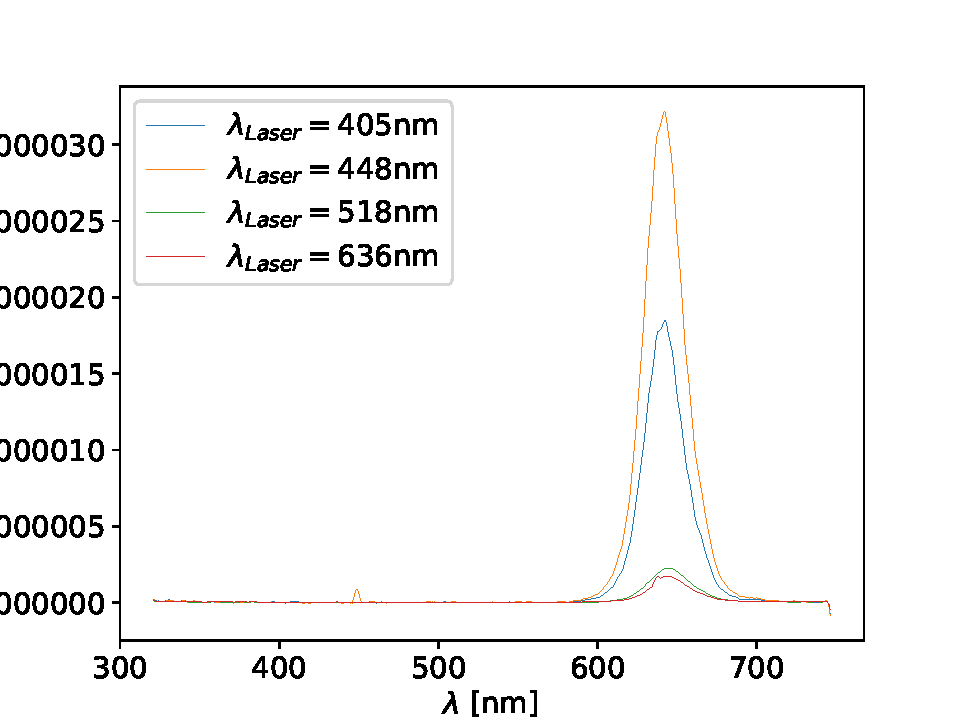
\includegraphics[width = 0.48\textwidth]{Probe_1_lambda.pdf}
    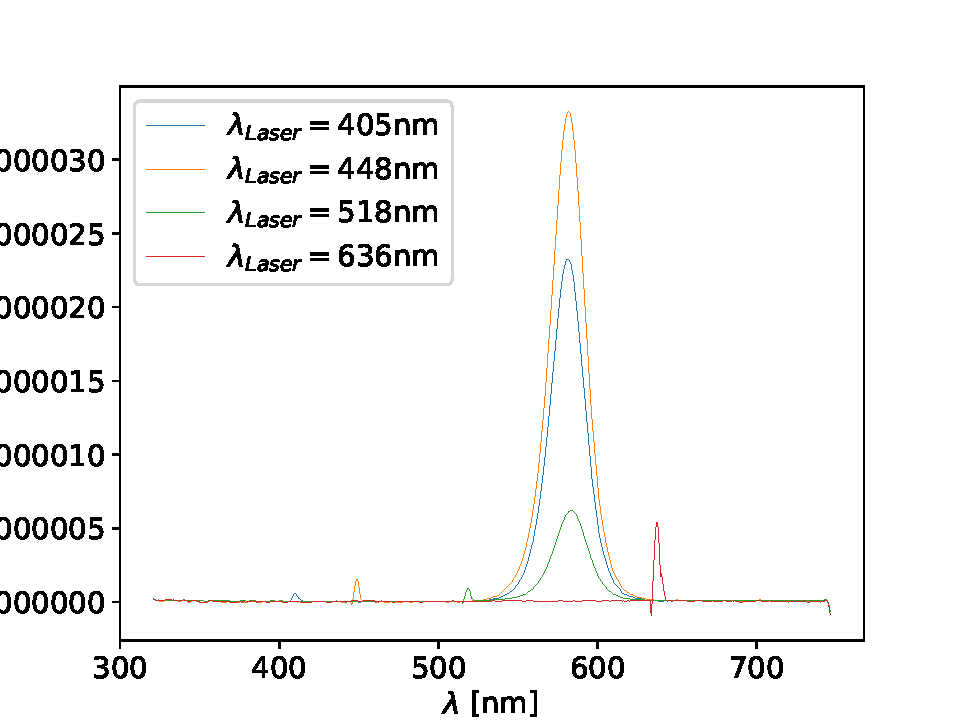
\includegraphics[width = 0.48\textwidth]{Probe_2_lambda.pdf}
    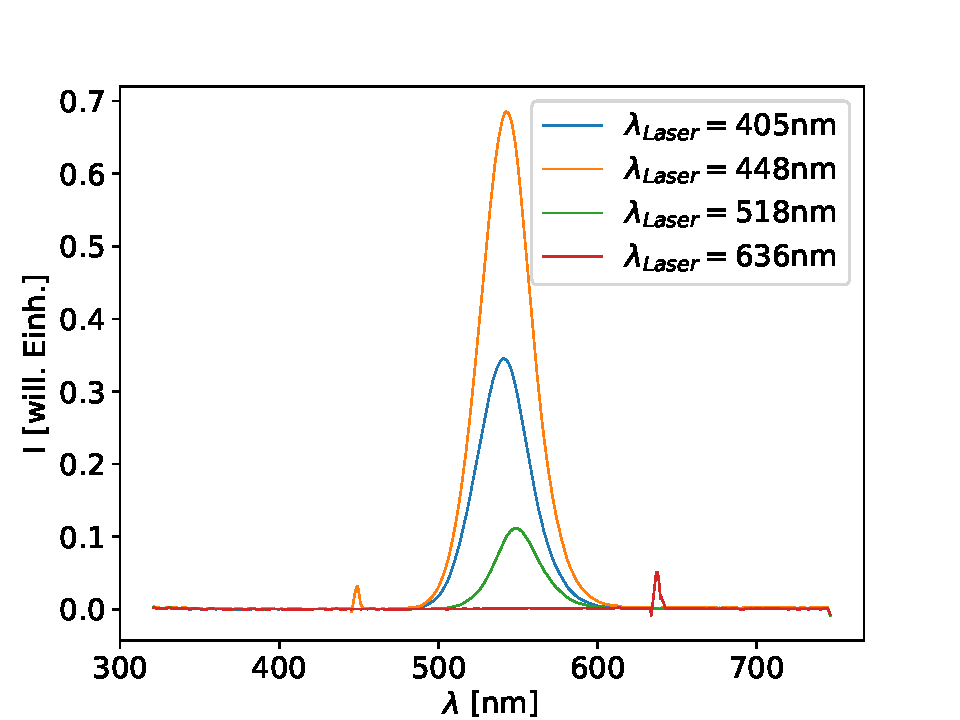
\includegraphics[width = 0.48\textwidth]{Probe_3_lambda.pdf}
    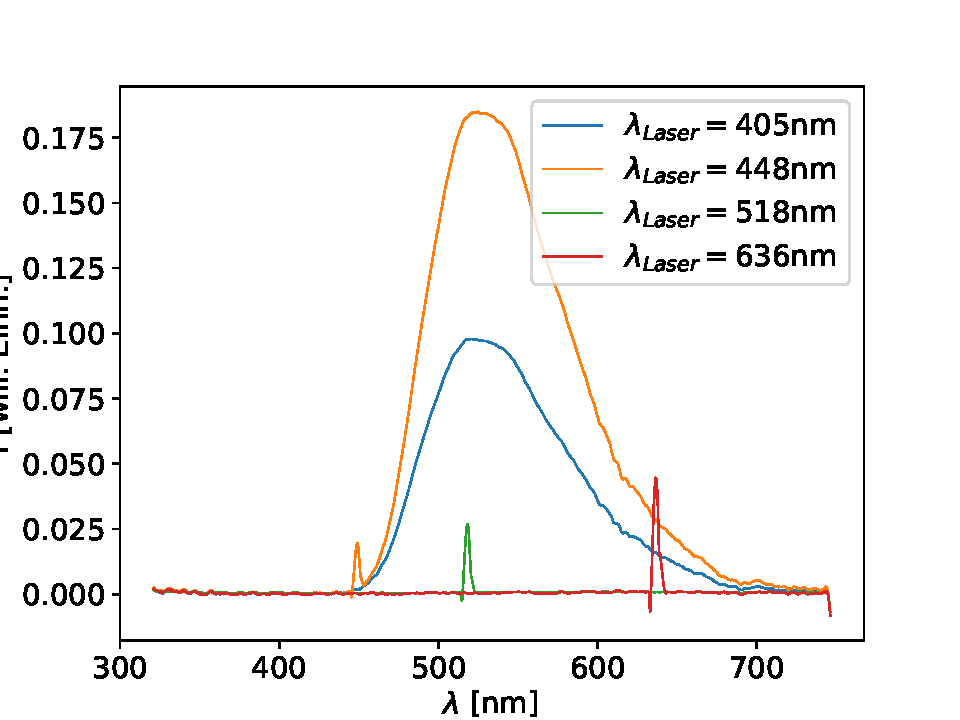
\includegraphics[width = 0.48\textwidth]{Probe_4_lambda.pdf}
    \caption{Photolumineszenzspektren der vier unteruschten Proben für die vier verschiedenen Anregungsenergie.}
    \label{fig:PLvsLambda}
    \end{figure}

    \FloatBarrier

